\documentclass[a4paper]{article}        % Standaard een kolom layout
\usepackage[english]{babel}             % Stel woordafbrekingen en referentienamen in
\usepackage{graphicx}                   % Afbeeldingen weergeven
\usepackage{float}                      % Figuren op plaats waar ze gedefinieerd staan: [H]
\usepackage{lmodern}                     % Lettertype instellen op Helvetica
\usepackage[T1]{fontenc}
\usepackage[hidelinks]{hyperref}        % Referenties aanklikbaar in PDF, geen kaders rond weergeven
\usepackage{siunitx}                    % SI unit symbolen
\usepackage{amsmath}                    % Matrices en vergelijkingen
\usepackage{subcaption}                 % Subfiguren
\usepackage[parfill]{parskip}			% Niet inspringen aan begin alinea


\title{Hardware Design Project\\ Designing a drone positioning sensor}
\author{Laurens Bogaert\\Thomas Deckmyn\\Zeger Van de Vannet}
\date{\today}

\begin{document}
\maketitle

% Inhoudstafel
\newpage
  \tableofcontents
\newpage

\section{Antenna Design}
	
	For the indoor localisation of the drones we use the TIME DOMAIN\texttrademark PulsOn 400 UWB module in coöperation with a STM32 microcontroller to run the Unscented Kalman Filter algorithm. The UWB modules are already equipped with a TIME DOMAIN\texttrademark Broadspec UWB Antenna, a dipole that is omnidirectional in the azimuth plane. We will use the specifications of this antenna as design parameters for or own UWB antenna. The criticial design parameters are listed below. 

	\begin{itemize}
		\item Radiate in the $\SI{3.1}{\giga\hertz}$ - $\SI{5.3}{\giga\hertz}$ band
		\item Nominal gain $\approx \SI{3}{\decibel}$
		\item Linear phase characteristic
		\item Efficiency $\approx$ 90\%	

	\end{itemize}

	\subsection{Antenna Topology and Design}
	\label{subsec:ant_design}

	At first we experiment with a few conventional UWB topologies like a bow tie and a bar-bell shape (see Figure \ref{fig:topologies}). After optimalisation and simulation in ADS, we conclude that the simulated S-paramters and gain are not compliant with the design parameters above. Obtaining a linear phase characteristic with these topologies proves to be very hard as well.  

		\begin{figure}[H]
		\begin{subfigure}{0.5\textwidth}
			\centering
			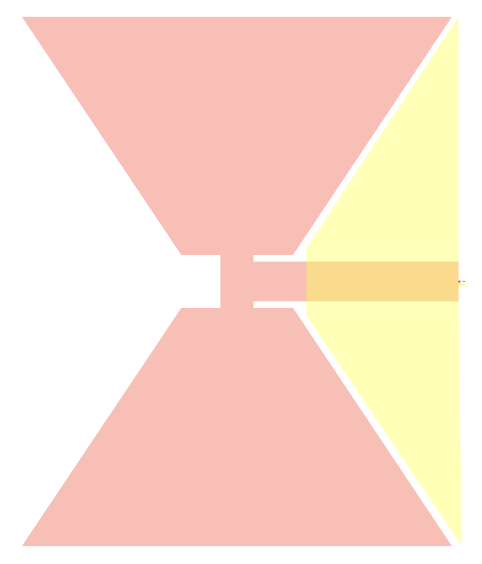
\includegraphics[width=0.5\textwidth,height=85px]{images/antenna/bow_tie.png}
			\caption{Bow Tie Topology}
		\end{subfigure}
		\begin{subfigure}{0.5\textwidth}
			\centering
			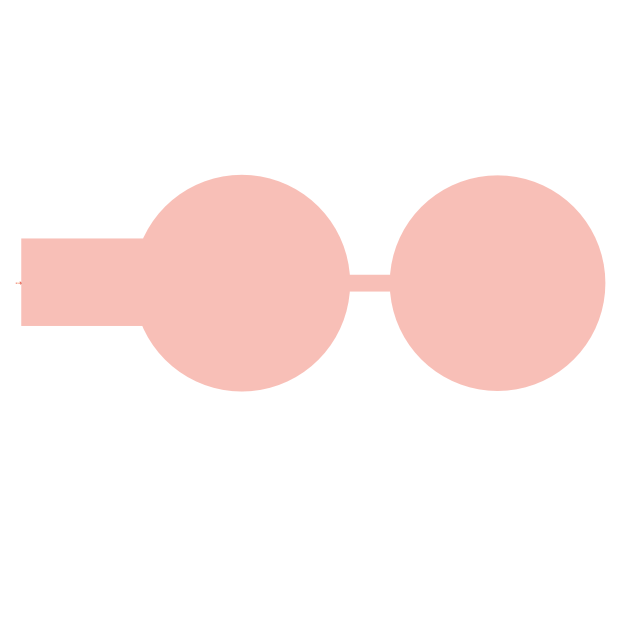
\includegraphics[width=0.5\textwidth]{images/antenna/bar_bell.png}
			\caption{Bar-Bell Topology}
		\end{subfigure}
		\caption{UWB Antenna Topologies}
		\label{fig:topologies}
		\end{figure} 

	The substrate material that is being used to desing the antenna is \textit{Black Foam} with a low relative permittivity $\epsilon_r = 1.495$. Because of this we encounter a practical problem with respect to the dimension of the antenna, i.e. if the antenna needs to be constructed with this substrate its dimension will be too large to mount on the drone. Thus for the remaining part of the design process we opt for an \textit{Aromated Polyurethane} substrate with a higher $\epsilon_r = 2.55$, which allows us to work with smaller dimensions while radiating in the same frequency band. 

	After experimenting with the exotic topologies mentioned above, we redo the design starting from a rectangular microstrip patch antenna. The length of the patch determines the resonance frequency of the device, while the width has an influence on the radiated power. A wider patch means less resonance resistance, hence more bandwidth and a higher efficiency. 
	We want the resonance frequency of the patch to be in the predefined frequency band $\SI{3.1}{\giga\hertz}$ - $\SI{5.3}{\giga\hertz}$ and thus choose $f_0 = \SI{4.2}{\giga\hertz}$. Using equation (\ref{eq:width_patch}) we calculate the desired width of the patch.
	\begin{equation} 
	L = \frac{c}{2 f_r \sqrt{\epsilon_r}}
	\label{eq:width_patch}
	\end{equation}

	The bandwidth of the antenna needs to be very wide, thus, as explained above, we would be tempted to increase the width of the patch to obtain a bigger bandwidth. Again, we are limited by the dimensions of the drone, because it needs to be fitted onto the drone and we don't want the antenna to interfere too mmuch with the aerodynamics. To increase the bandwidth we apply another technique, i.e. adding stairs to the rectangular patch and optimizing their dimensions to obtain the desired bandwidth. Also, we introduce a partial groundplane, of which we again optimize the dimensions, to realize an approximately flat $S_{11}$ and a linear phase characteristic in the wanted frequency band. The final antenna lay-out is shown in Figure \ref{fig:patch_stairs} and the optimized dimensions are given in Table.

	\begin{figure}[H]
	\centering
		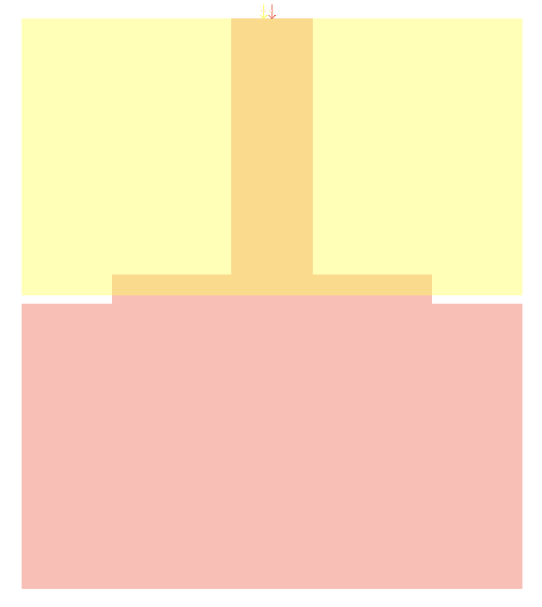
\includegraphics[width=0.5\textwidth]{images/antenna/patch_stairs.png}
		\caption{Rectangular patch antenna with added stairs and partial ground plane}
		\label{fig:patch_stairs}
	\end{figure}

	\begin{table}[H]
	\centering
	\begin{tabular}{|c|c|}
		\hline
		\multicolumn{2}{|c|}{\textbf{Antenna}} \\ \hline
		L & $\SI{20.5}{\milli\meter}$ \\ \hline
		W & $\SI{36}{\milli\meter}$ \\ \hline
		$W_{stair}$ & $\SI{8.6}{\milli\meter}$ \\ \hline
		$H_{stair}$ & $\SI{2.1}{\milli\meter}$ \\ \hline
		\multicolumn{2}{|c|}{\textbf{Ground Plane}} \\ \hline
		L & $\SI{19.2}{\milli\meter}$ \\ \hline
		W & $\SI{36}{\milli\meter}$ \\ \hline 
	\end{tabular}
	\caption{Optimized dimensions for antenna and partial ground plane}
	\label{tab:dimensions}
	\end{table}

	\subsection{Simulation}
		While designing the antenna, simulations in ADS are used to confirm that the antenna's characteristics are as desired. In this section we will discuss the simulation results of the final design, as explained in the previous section \ref{subsec:ant_design}. 

		\begin{figure}[H]
		\begin{subfigure}{0.5\textwidth}
		\centering
			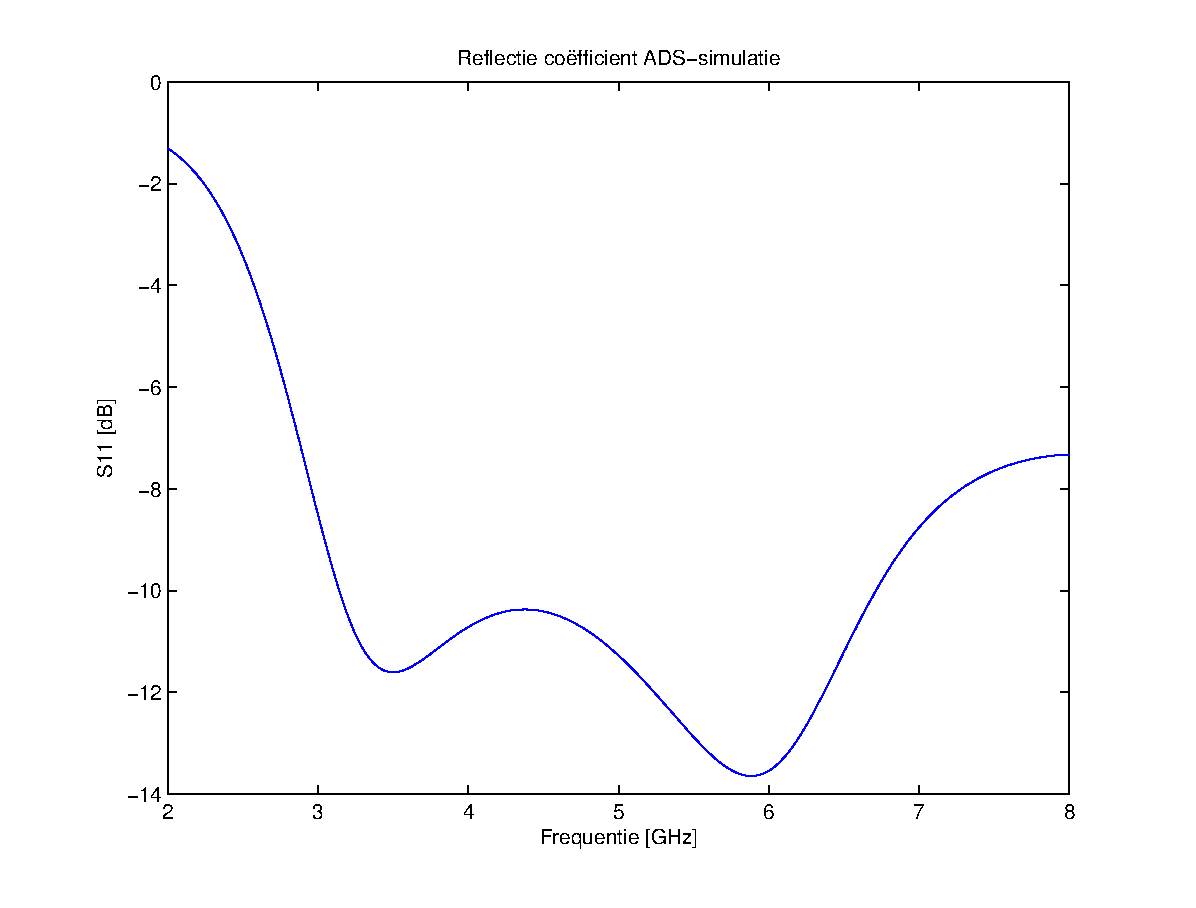
\includegraphics[width=\textwidth]{../presentation/images/S11_ADS_sim.eps}
			\caption{Simulated $S_{11}$}
		\end{subfigure}
		\begin{subfigure}{0.5\textwidth}
		\centering
			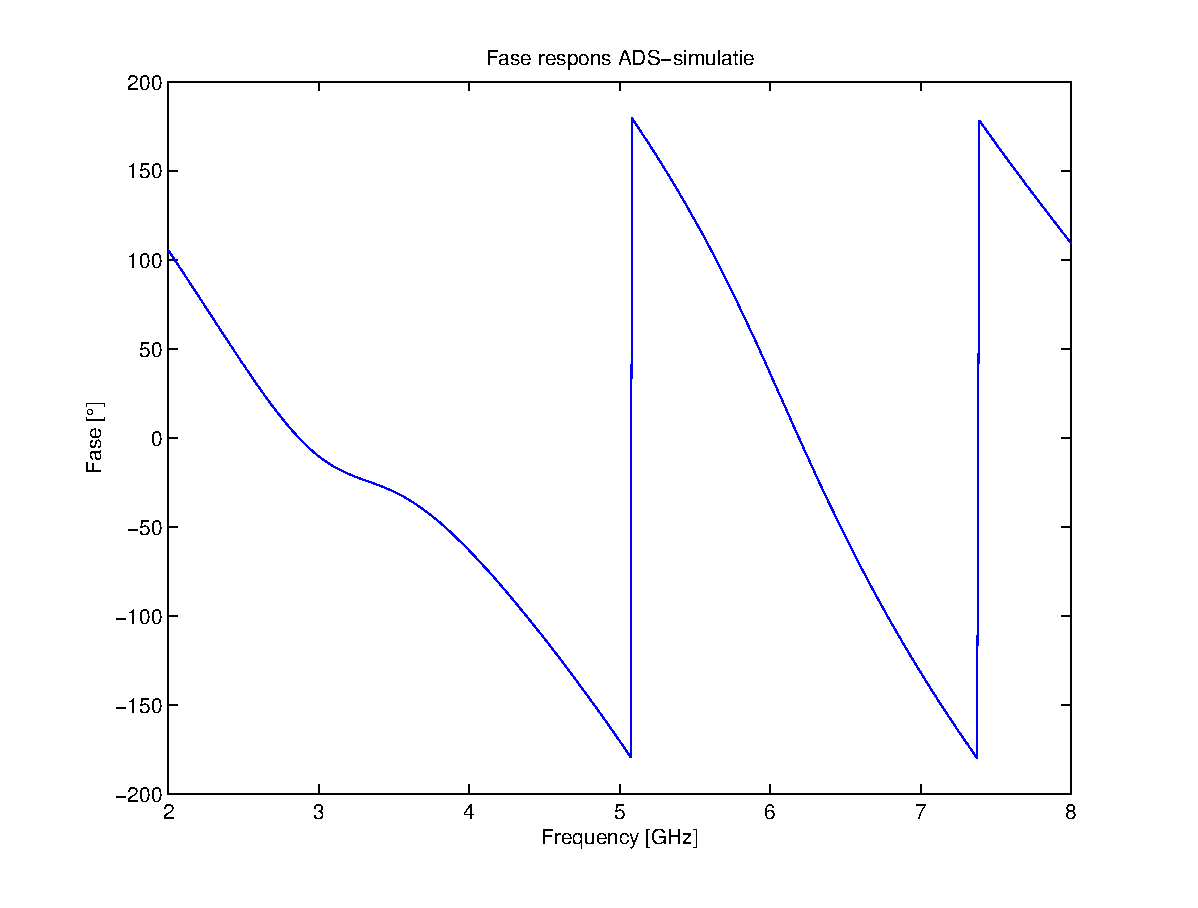
\includegraphics[width=\textwidth]{../presentation/images/fase_respons_ADS_sim.eps}
			\caption{Simulated phase respons}
		\end{subfigure}
		\caption{Simulated characteristics for designed UWB antenna}
		\label{fig:S11_phase_design}
		\end{figure}

		Figure \ref{fig:S11_phase_design} shows that the $S_{11}$-parameter is below $\SI{-10}{\decibel}$, and relatively flat, in the desired frequency band. 

	\subsection{Measurements}




\section{Location Algorithm}
	A first algorithm that can be used to determine the position of the drone is the \textit{Least Mean Square} algorithm. We will elaborate on this first and then compare the performance to the Unscented Kalman Filter, which will be used in the final system. 

	\subsection{Least Mean Square}
	\label{subsec:LMS}

		The LMS algorithm uses the distances between the drone and a number of well-known anchor points to determine the position. The UWB antenna mounted on the drone broadcasts a very short pulse to the anchors, which will return the same pulse when it is received. The board on the drone measures the time between sending the pulse and receiving it back. Because the propagation speed of the pulse through air and the time it takes to process the pulse at the anchors are known, the distance to the anchor points can be determined as follows:

		\begin{equation}
		\centering
			t_{roundtrip} = 2t_{propagation} + t_{process}
		\end{equation} 

		Because the time to process the pulse at the anchor is known, we can calculate the time it takes to bridge the distance between the drone and the anchor point. With c the speed of light ($\SI{3e8}{\meter\per\second}$) this results in an expression for the distance to anchor point i:

		\begin{equation}
		\centering
			d_i = c*t_{propagation}
		\end{equation}

		With $\vec{\textbf{x}}$ denoting the position vector $\begin{bmatrix} x & y & z \end{bmatrix}$ of the drone and $\vec{\textbf{x}_i}$ the position vector $\begin{bmatrix} x_i & y_i & z_i \end{bmatrix}$ of the $i^{th}$ anchor point, this distance can also be expressed as follows:

		\begin{align*}
		\centering
			d_i^2 &= (\vec{\textbf{x}} - \vec{\textbf{x}_i})(\vec{\textbf{x}} - \vec{\textbf{x}_i})^T \\
			&= x^2 - 2x_ix + x_i^2 + y^2 - 2y_iy + y_i^2 + z^2 - 2z_iz + z_i^2
		\end{align*}

		This equation is not linear in x, y and z and therefore it is hard to extract the position vector. With $d_N$ the distance to the $N^{th}$ anchor, the equation can be linearized as follows:

		\begin{align*}
		\centering
			d_i^2 - d_N^2 &= x^2 - 2x_ix + x_i^2 + y^2 - 2y_iy + y_i^2 + z^2 - 2z_iz + z_i^2 - d_N^2 \\
				&= 2x(x_N - x_i) + 2y(y_N - y_i) + 2z(z_N- z_i)+ (x_i^2 - x_N^2) + (y_i^2 - y_N^2)  + (z_i^2 - z_N^2) 
		\end{align*}

		This yields a matrix representation of the form $\textbf{A}\vec{\textbf{x}} = \textbf{B}$ which can be solved for the position vector $\vec{\textbf{x}}$.


	% subsection LMS (end)


\section{PCB Design}
  In order to process the measurements and determine the position of the drone, a microcontroller is used. We will use one from the STM32F4-series, which has a 32-bit ARM processor. A PCB is designed to contain the microcontroller, as well as power supply and peripheral connections.
The controller communicates with the RCM-controller over the UART-protocol, and can use the UWB-antenna for communication purposes as well as for ranging.
This way the microcontroller can report positioning data to a monitoring station.
Further connections include multiple means of supplying power to the microcontroller, either the power can be drawn from the drone itself, or it can be powered by an external battery.
A programming interface is also provided.
All IO-pins are ESD-protected using Zener diodes.
  
\end{document}

